\begin{figure}[htpb]
	\centering\capstart{}
	\subfloat[\(\Re{\pixel{\convolution{f_{A}}{g}}}\)]{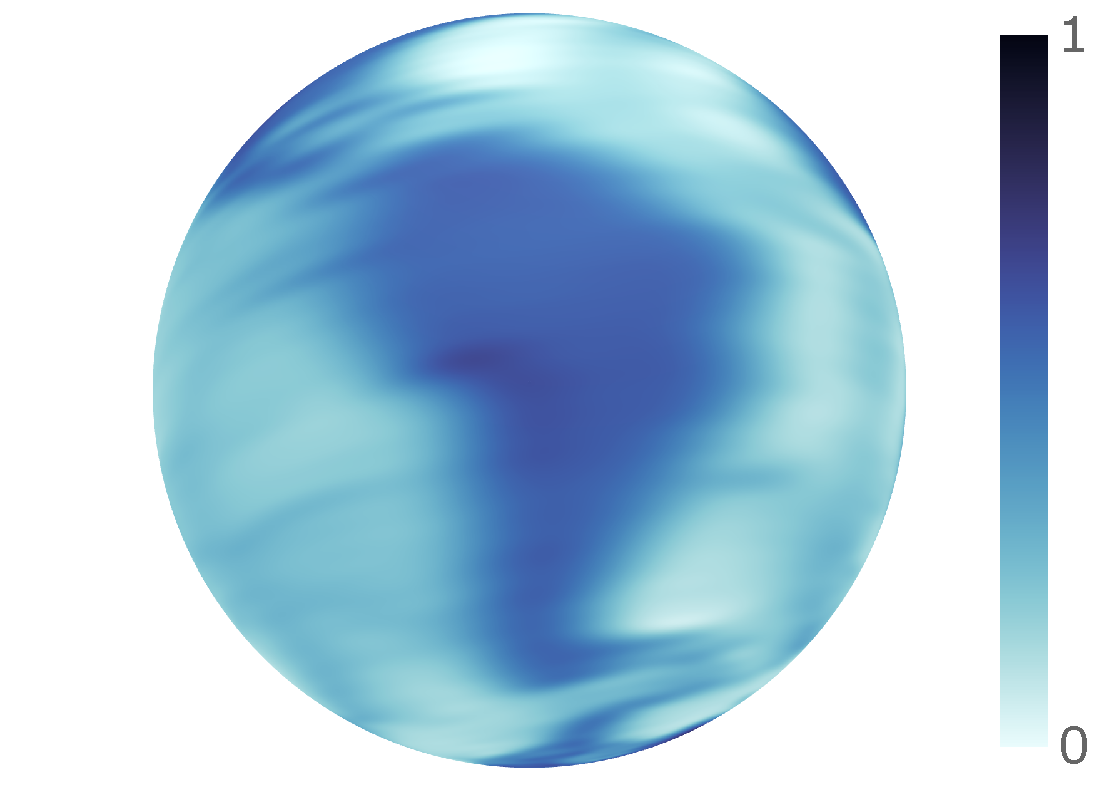
\includegraphics[trim={23 7 3 6},clip,width=.5\textwidth]{harmonic_gaussian_100lsig_10msig_L128_convolved_earth_L128_res512_real_norm.pdf}}
	\hfill
	\subfloat[\(\Re{\pixel{\convolution{f_{B}}{g}}}\)]{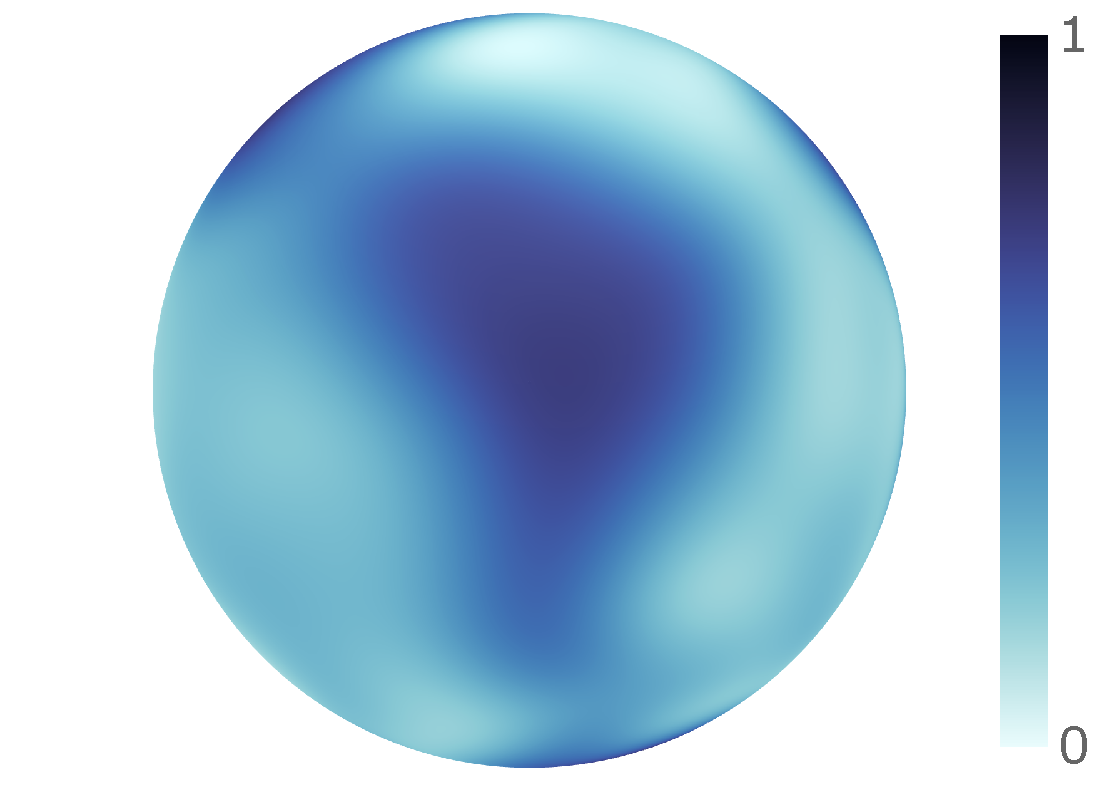
\includegraphics[trim={23 7 3 6},clip,width=.5\textwidth]{harmonic_gaussian_10lsig_10msig_L128_convolved_earth_L128_res512_real_norm.pdf}}
	\caption[
		Two harmonic Gaussians convolved with a map of the Earth
	]{
		The real part of the sifting convolution between the EGM2008 dataset and the harmonic Gaussian, rotated to view of South America (bandlimited at \(L=128\)).
		Panel (a) corresponds to a more elongated kernel \(f_{A}\), where \((\sigma_{\ell},\sigma_{m}) = (10^{2}, 10^{1})\); whereas panel (b) corresponds to a more symmetric kernel \(f_{B}\), where \((\sigma_{\ell},\sigma_{m}) = (10^{1}, 10^{1})\).
		As expected, the resultant sifting convolved Earth map exhibits greater anisotropic smoothing in panel (a) than in panel (b).
		It is clear that the sifting convolution supports directional kernels to perform anisotropic filtering (smoothing), while the output remains on the sphere.
		The colour is between zero and one, reflecting the scaled intensity of the field.
	}\label{fig:chapter2_convolved}
\end{figure}
